\section{Design and Development}

\subsection{Technologies}
\subsubsection{AprilTag}
AprilTags are QR-like codes that allow a calibrated camera to localize a known tag in an image relative to the camera. They do this by being unique orientation asymmetric patterns that are easy for a camera to recognize and orient. Knowing the real-world size of the tag they can then find the location and orientation of the tag relative to a camera. \cite{DetectAprilDemo} \cite{AprilTagRepo}


\subsection{Design}

In general, the design of the Simulink model follows the flow chart in Figure \ref{Fig:Model_Flowchart}. We used a main control switch to command the home position(input 1), camera position(input 2), or execute the pick-and-place motion(input 3). The pick-and-place motion was controlled by a counter that would start when the input to the control switch was 3 and would then count from 1 to 6 for each of the different states the arm should be in. This sequence can be seen in Figure \ref{Fig:Model_Flowchart} in the Counter Sequence sub-block where the numbers on the transitions indicate which position and gripper state is chosen for each value of the counter.

\begin{figure}[htb]
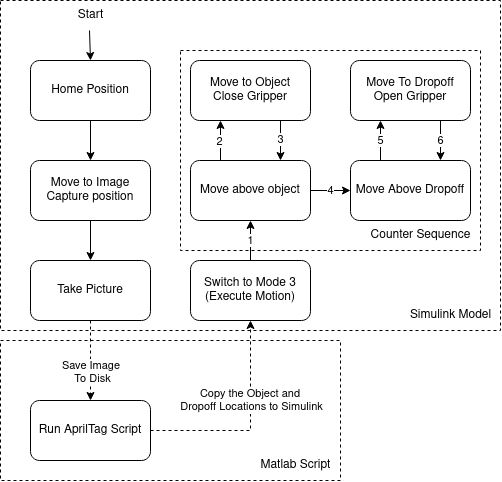
\includegraphics[width=8cm]{Figures/IntroRob_Final_Project_StateMachine_v2.drawio.png}
\caption{Model Flowchart}
\label{Fig:Model_Flowchart}
\centering
\end{figure}



\subsection{Matrix Mathematics}
Using Figure \ref{Fig:QARM_Coord}, the homogeneous transformation matrix (HTM) of the base to the ArilTag can be found by multiplying intermediate transformation matrices together as shown in equation \ref{Eqn:Tag2Base}, where \({}^{base}_{w}T\) is the HTM of the wrist with respect to the base, and \({}^{w}_{cam}T\) is the HTM of the camera with respect to the wrist, and \({}^{cam}_{tag}T\). 

\begin{equation}
\label{Eqn:Tag2Base}
{}^{base}_{tag}T = {}^{base}_{w}T\times{}^{w}_{cam}T\times{}^{cam}_{tag}T   
\end{equation}

The AprilTag's position, \({}^{base}_{tag}P\) is defined as elements (1:3,4) of \({}^{base}_{tag}T\). Once the position of the AprilTag with relation to the base is determined, inverse kinematics can be used to calculate possible solutions the QArm can take to pick up the object and place it at the drop-off location. For this project, the first set of solutions was used in the motion of the QArm. 

\begin{figure}[htb]
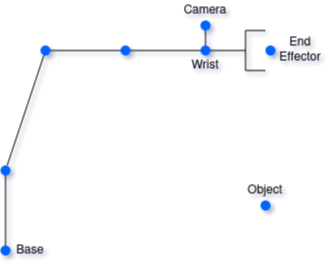
\includegraphics[width=8cm]{Figures/IntroRob_Final_Project_Coordinates.drawio.png}
\caption{QArm Coordinate System}
\centering
\label{Fig:QARM_Coord}
\end{figure}
